\documentclass[12pt]{article}
\usepackage[UTF8]{ctex}
\usepackage{graphicx}
\usepackage[utf8]{inputenc}
\usepackage{CJKutf8}
\usepackage{fancyhdr}

\pagestyle{fancy}
\lhead{《数学欣赏》课程论文}
\rhead{敖冠舒 \ 叶昊宇}


\baselineskip=15pt
\textwidth 140mm
\textheight 225mm
\oddsidemargin 5.6mm
\evensidemargin 5.6mm
\parindent=2\ccwd

\topmargin -5mm



\begin{document}

\title
{\bf\Large 图像去雾算法分析}
\date{\small 2022.12}
\author{\small 敖冠舒(电子信息学院) \and \small 叶昊宇(数学与统计学院)}
\maketitle

\thispagestyle{fancy}  

\begin{abstract}
本文介绍了图像去雾算法产生的背景算法面临的难点,对基于图像增强的图像去雾算法、基于物理模型的图像去雾算法和基于深度学习的去雾算法三种主要的去雾算法及其细分算法的原理、实现、优势、劣势进行了简要分析,同时指出了几种图像去雾算法存在的问题和未来的改进方向,并展望图像去雾算法在未来能得到更广泛的应用。
\end{abstract}

\section{引言}
\subsection{概述}

现代社会的发展总是伴随着环境污染,雾霾现象发生越来越频繁,很大程度上影响我们的生活。雾霾是由空气中的灰尘和烟雾等小的漂浮颗粒产生的常见大气现象,这些漂浮的颗粒极大地吸收和散射光,导致拍摄图像质量下降。在雾霾影响下,视频监控,远程感应,自动驾驶等许多实际应用很容易受到威胁,检测和识别等高级计算机视觉任务很难完成。

现有的图像采集设备对外界环境的干扰非常敏感,在雾霾环境中,获取的户外图像往往退化严重,主要表现为场景特征信息模糊、对比度低、色彩失真,不利于计算机视觉系统对图像真实特征的提取,从而影响其后续的分析、理解、识别等一系列处理,很大程度上降低了视觉系统的实际应用性能,限制了图像的应用价值。因此需要去雾算法来对此类低质图片进行预处理,保证系统的正常运转。

正因如此,图像去雾越来越成为一种重要的技术,有极高的研究价值,同时也是一项充满挑战性的课题。图像去雾是以满足特定条件下应用需求为目的,通过对有雾图像进行分析和预处理,突出图像中的细节信息使之更加适合人机识别的一种图像预处理方法。

目前图像去雾算法主要包括基于图像增强的图像去雾算法、基于物理模型的图像去雾算法和基于深度学习的去雾算法三种。

\subsection{算法难点}
图像去雾领域存在的难点问题主要表现在如下三个方面:

\textbf{雾图特征有限}:有雾图像由于受到雾气成像环境的干扰,其亮度、纹理、轮廓、形状等特征都存在不同程度的损失。图像增强类算法大多以提高图像清晰度为目标,由于没有考虑到雾图成像的原理,全局或局部的增强处理结果容易出现过增强。基于大气散射模型的图像去雾方法是依据大气成像的机理,从输入雾图中复原出清晰图像。但成像模型参数众多,实际成像环境很复杂,加上可利用的雾图特征十分有限,依据模型求解无雾图像也并非易事。因此,如何利用有限的图像特征执行有效的图像去雾仍然是具有挑战性的问题。

\textbf{实时处理问题}:如果雾图增强或复原花费的计算或存储开销过大,势必极大影响应用系统的实时工作。但现有的许多图像增强类算法或者基于物理模型的方法,为了获得较好的复原效果,往往具有较大的计算复杂度,不适合部署在实际的视觉系统上。而基于深度学习的方法虽能降低一些时间开销,但相对于实时处理来说仍有一定差距。因此,如何在确保图像去雾效果的同时,提高图像去雾的速度,满足应用实时处理的需求,是目前主要的研究目标。

\textbf{普适性问题}:算法面临的最大问题是对不同类型的雾图难以获得一致的增强或复原质量。不同图像对应的拍摄场景往往区别很大,因此,利用统一的模型去复原不同类型场景的图像是难以达到一致的去雾效果的,深度学习目前看来是可以通过大量数据的训练来解决此问题,但总的来说,图像去雾算法的普适性面临很大的挑战。

\section{基于图像增强的去雾算法}

基于图像增强的去雾算法通常不考虑雾天图像降质的原因,通过对有雾图像进行处理,增强有雾图像的全局特性或局部特性,使得图像质量得以改善,丰富图像中的信息量。目前比较典型的图像增强算法主要包括基于直方图均衡化的去雾算法、同态滤波算法以及基于Retinex的去雾算法。

\subsection{基于直方图均衡化的图像去雾算法}

直方图均衡化算法的基本思想是通过直方图均衡化来扩大原有雾图像的灰度范围,改善原有雾图像对比度低的问题。在图像处理中, 经常用到直方图, 如颜色直方图、 灰度直方图等。图像的灰度直方图就描述了图像中灰度分布情况, 能够很直观的展示出图像中各个灰度级所占的多少。图像的灰度直方图是灰度级的函数, 描述的是图像中具有该灰度级的像素的个数: 其中, 横坐标是灰度级, 纵坐标是该灰度级出现的率。如下图所示:

\begin{figure}[h]
    \centering
    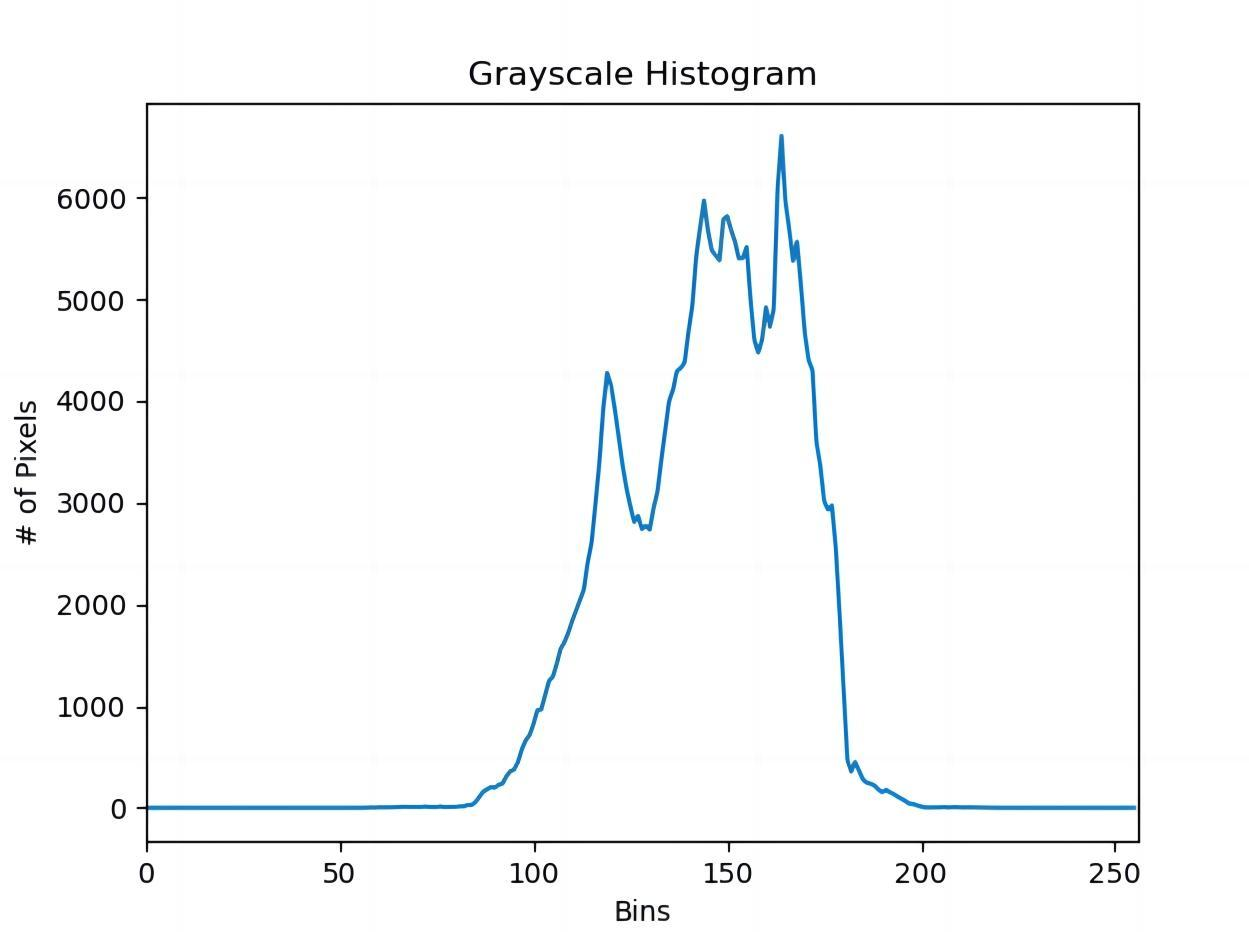
\includegraphics[width=0.7\textwidth]{pic/pic1.jpg}
    \caption{某幅图像的直方图,横轴表示灰度级,纵轴表示改灰度对应的像素数}
\end{figure}

直方图反映了图像中的灰度分布规律。 它描述每个灰度级具有的像素个数, 但不包含这些像素在图像中的位置信息。 图像直方图不关心像素所处的空间位置, 因此不受图像旋转和平移变化的影响, 可以作为图像的特征。任何一幅特定的图像都有唯一的直方图与之对应, 但不同的图像可以有相同的直方图。如果一幅图像有两个不相连的区域组成, 并且每个区域的直方图已知, 则整幅图像的直方图是该两个区域的直方图之和。如果需要将上图中灰度偏暗、偏亮或偏集中的直方图调整为灰度均匀分布的直方图,就需要用到直方图均衡化算法。

直方图均衡化(Histogram Equalization, HE)是一种增强图像对比度(Image Contrast)的方法,其主要思想是将一副图像的直方图分布通过累积分布函数变成近似均匀分布,从而增强图像的对比度。为了将原图像的亮度范围进行扩展, 需要一个映射函数, 将原图像的像素值均衡映射到新直方图中, 这个映射函数有两个条件:
\begin{itemize}
    \item 能打乱原有的像素值大小顺序, 映射后亮、 暗的大小关系不能改变
    \item 映射后必须在原有的范围内,即像素映射函数的值域应在0和255之间
\end{itemize}

综合以上两个条件,累积分布函数是个好的选择,因为累积分布函数是单调增函数(控制大小关系),并且值域是0到1(控制越界问题),所以直方图均衡化中使用的是累积分布函数。

直方图均衡化算法改善有雾图像对比度低的方式是使用全局均衡化或局部均衡化算法将图像的灰度范围扩大,从而提高图像的对比度来实现图像去雾的效果。该算法的一般步骤如下:

第一步:计算输入图像的灰度,记为$r_k$;

第二步:计算输入图像中第$k$个灰度级出现的概率,记为$P_r(r_k)$;
\begin{equation}
    P_r(r_k)=\frac{n_k}{n} \quad , \quad 0\leq r_k \leq 1 \quad k=0,1,\dots ,l-1
\end{equation}
其中,$n_k$为输入图像中灰度级为$k$的像素数量,$n$为输入图像的像素数量,$l$为灰度级的个数。

第三步:设变换函数为$T(r_k)$,根据积累分布函数的定义可以计算出概率累积值,即为均衡化后的图像灰度级,记为$s_k$:
\begin{equation}
    s_k=T(r_k)=\sum_{j=0}^{k}{P_r(r_j)}=\sum_{j=0}^{k}{\frac{n_j}{n}}
    \quad,\quad 0\leq r_k \leq 1 \quad , \quad k=0,1,\dots ,l-1
\end{equation}
其中,累积分布函数具有单调递增的特点。

全局直方图均衡化算法直接对有雾图像整体进行处理,算法简单易实现,比较适合整体偏亮或偏暗的有雾图像。但由于该算法未考虑图像的局部细节,不能适应输入图像的局部亮度特性,可能会导致增强后的图像灰度层次感较差。

当有雾图像中雾浓度分布均匀时,上述HE算法能够实现不错的去雾效果,但是当雾浓度分布不均匀时,HE算法的去雾效果不佳。自适应直方图均衡化算法(Adaptive Histogram Equalization, AHE)在上述HE算法上进一步改进,使用有雾图像中的局部直方图代替全局直方图来提高有雾图像的对比度,能够更好地恢复有雾图像的局部信息,适应性更强。但是AHE算法恢复的无雾清晰图像可能会出现噪声放大问题,当有雾图像中某区域包含大量相似的像素值时,该区域的直方图会出现不均衡的情况,AHE算法会将这种局部不均衡放大到整个图像,导致少量噪声被放大。

\subsection{基于同态滤波的图像去雾算法}

同态滤波是一种在频域内对图像进行对比度增强的算法。同态滤波算法将有雾图像的复原问题转换成增大有雾图像频域范围的问题,通过减少有雾图像中的低频信息,并相应增加图像中的高频信息,可以实现图像去雾的效果。

同态滤波算法是以照射反射模型为基础,将图像分为照射分量和反射分量,照射分量变化缓慢是图像的低频部分,反射分量变化较快是图像的高频部分。同态滤波算法通过减少低频信息增加高频信息,从而减少光照变化并锐化有雾图像细节来实现图像去雾的效果。

\begin{figure}[h]
    \centering
    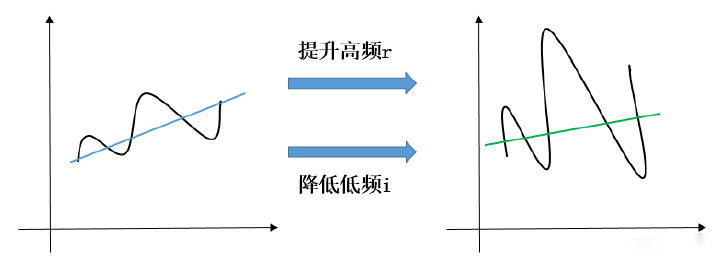
\includegraphics[width=0.7\textwidth]{pic/pic2.png}
    \caption{使用同态滤波法后,图像在频域内的变化}
\end{figure}

同态滤波法的主要步骤如下:

第一步:设一幅有雾图像为$f(x,y)$,将该图像表示为照射分量$i(x,y)$和反射分量$r(x,y)$的乘积,如下所示:

\begin{equation}
    f(x,y)=i(x,y)·r(x,y)
\end{equation}
其中,$i(x,y)$描述景物的照明,变化缓慢,是输入图像中的低频成分;$r(x,y)$描述景物的细节,变化迅速,是输入图像的高频成分。

第二步:对第一步中的式$(3)$两边分别取对数,可得到如下的$z(x,y)$:
\begin{equation}
    z(x,y)=\ln f(x,y) =\ln i(x,y) +\ln r(x,y)
\end{equation}

第三步:对第二步得到的式$(4)$进行傅里叶变换,可以得到如下$z(u,v)$:
\begin{equation}
    Z(u,v)=Fi(u,v) +Fr(u,v)
\end{equation}

第四步:对第三步得到的$Z(u,v)$进行滤波处理,可得到如下$S(u,v)$:
\begin{equation}
    S(u,v)=H(u,v)S(u,v)=H(u,v)·Fi(u,v) +H(u,v)·Fr(u,v)
\end{equation}
特别地,用来进行滤波处理的滤波器通常取如下形式:
\begin{equation}
    H(u,v)=(\gamma_H -\gamma_L)·H_{hp}(u,v)+\gamma_L
\end{equation}
其中,$\gamma_H$和$\gamma_L$两个参数用来调节滤波器的幅度范围,$H_{hp}$通常是高通滤波器。

第五步:对第四步中的式$(6)$进行反傅里叶变换,可以得到如下$s(x,y)$:
\begin{equation}
    s(x,y)=IDFT(S(u,v))
\end{equation}

第六步:对第五步中的式$(8)$两边取指数,可以得到经过同态滤波处理后的图像$g(x,y)$:
\begin{equation}
    g(x,y)=exp(s(x,y))=io(x,y)·ro(x,y)
\end{equation}

\subsection{基于Retinex理论的图像去雾算法}
Retinex是一种常用的建立在科学实验和科学分析基础上的图像增强方法,它是Edwin.H.Land于1963年提出的。就跟Matlab是由Matrix和Laboratory合成的一样,Retinex也是由两个单词合成的一个词语,他们分别是retina 和cortex,即:视网膜和皮层。Land的retinex模式是建立在以下三个假设之上的:
\begin{itemize}
    \item 真实世界是无颜色的,我们所感知的颜色是光与物质的相互作用的结果
    \item 每一颜色区域由给定波长的红、绿、蓝三原色构成的
    \item 三原色决定了每个单位区域的颜色
\end{itemize}


Retinex理论的基础理论是物体的颜色是由物体对长波(红色)、中波(绿色)、短波(蓝色)光线的反射能力来决定的,而不是由反射光强度的绝对值来决定的,物体的色彩不受光照非均匀性的影响,具有一致性,即Retinex是以色感一致性(颜色恒常性)为基础的。不同于传统的线性、非线性的只能增强图像某一类特征的方法,Retinex可以在动态范围压缩、边缘增强和颜色恒常三个方面达到平衡,因此可以对各种不同类型的图像进行自适应的增强。40多年来,研究人员模仿人类视觉系统发展了Retinex算法,从单尺度Retinex算法,改进成多尺度加权平均的MSR算法,再发展成彩色恢复多尺度MSRCR算法。

Retinex 算法的一般步骤如下:

第一步:将一幅有雾图像$S(x,y)$表示成反射分量$R(x,y)$和亮度分量$L(x,y)$的乘积形式:

\begin{equation}
    S(x,y)=R(x,y)·L(x,y)
\end{equation}

第二步:对第一步中的式$(10)$两边分别取对数并移项,结果如下:
\begin{equation}
    \ln(R(x,y))=\ln(S(x,y))-\ln(L(x,y))
\end{equation}

第三步:对式$(11)$去除亮度分量$L(x,y)$,求得反射分量$R(u,v)$,从而得到增强后的图像,实现原图像的去雾处理。其中,计算$L(x,y)$是实现去雾的关键,在单尺度Retinex增强算法(Single-Scale Retine,SSR)中,提到高斯卷积函数可用于估计$L(x,y)$,可以表示为:
\begin{equation}
    L(x,y)=S(x,y)*H(x,y)
\end{equation}
\begin{equation}
    H(x,y)=u·exp(-\frac{x^2+y^2}{\sigma^2})
\end{equation}
其中,$*$为卷积操作,$u$为归一化值,$\sigma$为高斯环绕尺度参数。

可以得到:
\begin{equation}
    \ln(R_c(x,y))=\ln(S_c(x,y))-\ln(S_c(x,y) * H(x,y))
\end{equation}
其中,$c$表示彩色图像RGB颜色空间中的某一颜色通道。

当$\sigma$参数取合适值时,SSR算法能够实现良好的去雾效果,但是该算法容易受到高斯环绕尺度参数$\sigma$的影响。当$\sigma$较大时,SSR算法对图像细节恢复不够,当$\sigma$较小时,经过处理的图像会产生颜色失真。因此,为解决SSR算法对尺度参数$\sigma$的依赖,多尺度Retinex算法(Multi-Scale Retinex,MSR)被提出,以彩色图像为例,对RGB三个通道分别进行不同尺度的滤波,结果如下:
\begin{equation}
    \ln(R_{MSR}(x,y))=\sum_{i=1}^{3}{w_i ·\ln(R_{\sigma i}(x,y))}
\end{equation}
其中,$w_1$、$w_2$和$w_3$均为常数,$R_{\sigma 1}(x,y)$、$R_{\sigma 2}(x,y)$和$R_{\sigma 3}(x,y)$分别为RGB图像三个颜色通道的反射分量,每个颜色通道对应不同的$\sigma$值。MSR算法虽然解决了SSR算法对尺度参数$\sigma$的依赖,但是RGB三通道使用不同高斯环绕尺度参数$\sigma$的高斯滤波器进行滤波后,可能导致图像出现颜色失真。


\section{基于大气散射模型的去雾算法}


基于物理模型的去雾算法分析了雾霾天气导致原始图像降质的原因,通过建立物理模型来恢复无雾图像。几乎所有的基于物理模型的去雾算法均通过大气散射模型实现图像去雾,其模型示意图如图3所示。
\begin{figure}[h]
    \centering
    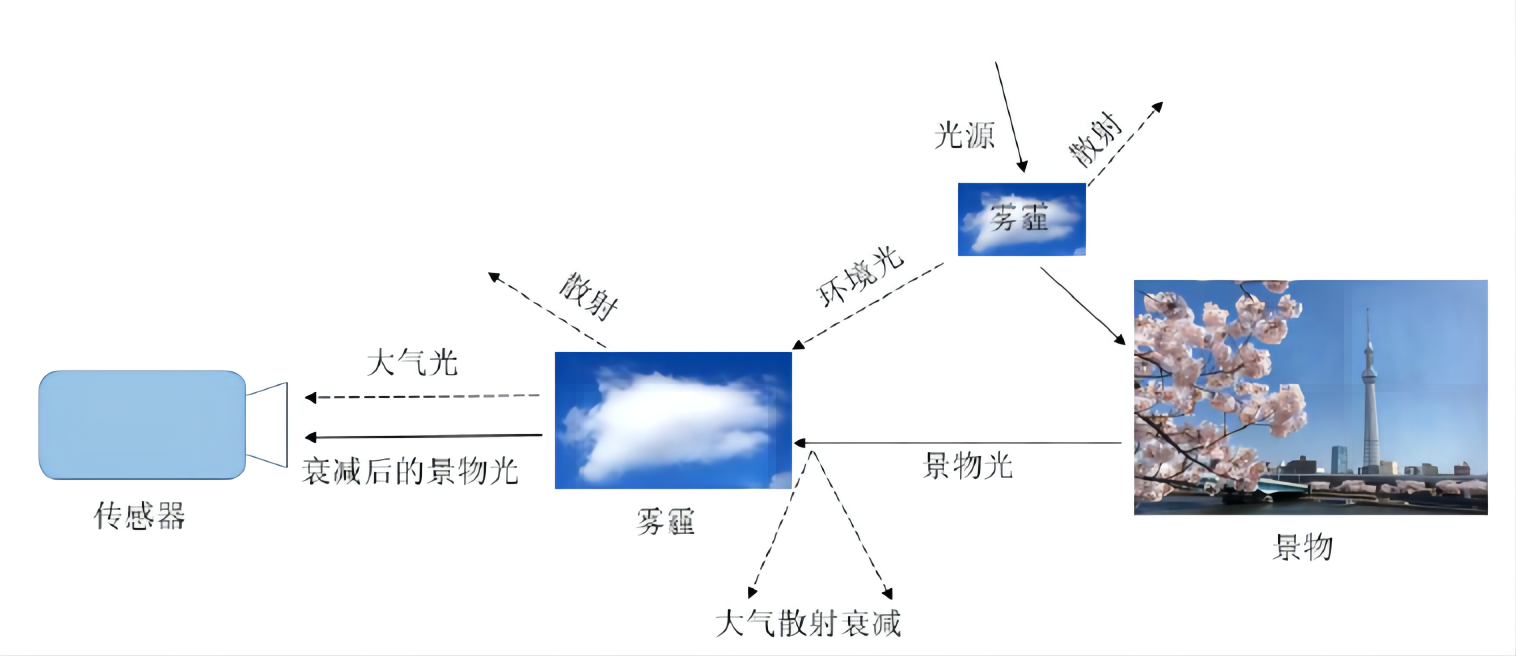
\includegraphics[width=\textwidth]{pic/pic3.png}
    \caption{大气散射模型示意图}
\end{figure}


大气散射模型对雾天图像的成像过程进行建模,具体地,有雾图像I(x)可以表示成如下形式:
\begin{equation}
    I(x)=J(x) t(x)+A(1-t(x))
\end{equation}
其中, $x$是$I(x)$中的某一像素点,$I(x)$是经过大气粒子散射到达传感器的有雾图像,$J(x)$是未被大气粒子散射之前的清晰无雾图像,$A$是大气光照,$t(x)$是场景透射率,可以表示成如下形式:
\begin{equation}
    t(x)=e^{-\beta d(x)}
\end{equation}
其中$\beta$是大气散射系数,$d(x)$表示场景深度。

基于大气散射模型实现图像去雾的关键是求解两个未知参数透射率值$t(x)$和大气光照值$A$。再将透射率$t(x)$的估计值和大气光照$A$的估计值代入大气散射模型公式,即可得到恢复的无雾图像。

\subsection{基于暗通道先验的图像去雾算法}
在何恺明博士的论文中提出利用暗通道先验对单张图像进行雾去除。在原论文中提到暗通道先验的概念是通过对户外无雾图像的一种统计结果得来。作者在论文中统计了5000多幅图像的特征,发现对于一幅彩色图像在绝大多数非天空的局部区域里,某一些像素总会有至少一个颜色通道具有很低的值。换言之,该区域光强度的最小值是个很小的数。暗通道的数学定义为对于任意的输入图像$J$,其暗通道可以用下式表达:
\begin{equation}
J^{dark}(x)=\min _{y \in \Omega(x)}\left(\min _{c \in(r, g, b)} J^{c}(y)\right)
\end{equation}
其中,$J^c$为清晰图像$J(x)$三种色彩通道,$\Omega(x)$为图像$J(x)$中以像素$x$为中心的某一窗口,窗口大小可以根据实际情况适当调整。上式意思为:一个暗通道的值等于取一个局部窗口中每个像素点三个通道中最小值组成的集合的最小值。通过对整幅图像进行上面的操作便可以得到一幅暗通道图。作者通过大量的统计得到的先验理论指出:
\begin{equation}
    J^{dark} \to 0
\end{equation}
即对于无雾的非天空部分图像的暗通道值总是趋于0,实际生活中造成上面情况主要有三个因素:
\begin{itemize}
    \item 汽车、建筑物和城市中玻璃窗户的阴影,或者是树叶、树与岩石等自然景观的投影
    \item 色彩鲜艳的物体或表面,在RGB的三个通道中有些通道的值很低(比如绿色的草地、红色或黄色的花朵、蓝色的水面)
    \item 颜色较暗的物体或者表面,例如灰暗色的树干和石头
\end{itemize}
总之,自然景物中到处都是阴影或者彩色,这些景物的图像的暗原色总是比较灰暗的。而相反的,对于有雾的图像来说其暗通道值不是趋于0。这里还需要说明的是何恺明的论文理论对于处理带有天空部分的雾图像的效果是不够好的。


上式即为暗通道先验算法的原理,基于暗通道先验和大气散射模型来实现图像去雾的DCP(Dark Channel Prior,DCP) 算法的一般步骤如下:

第一步:估计并细化透射率值,具体过程如下:假设全局大气光照$A$已知,并且是正值,对大气散射模型公式两边分别除以$A^c$:
\begin{equation}
    \frac{I^{c}(x)}{A^{c}}=t(x) \frac{J^{c}(x)}{A^{c}}+1-t(x), c \in(r, g, b)
\end{equation}
对上式进行最小化,得到:
\begin{equation}
    \min _{y \in \Omega(x)}\left(\min _{c} \frac{I^{c}(y)}{A^{c}}\right)=\tilde{t}(x) \min _{y \in \Omega(x)}\left(\min _{c} \frac{J^{c}(y)}{A^{c}}\right)+1-\tilde{t}(x)
\end{equation}
在上式中,$t(x)$在一个很小的邻域内是常量,因此可以不放在最小化操作内。并且,无雾图像$J^c$的暗通道值为0,可以得到:
\begin{equation}
    J^{dark}(x)=\min _{y \in \Omega(x)}\left(\min _{c \in(r, g, b)} J^{c}(y)\right)=0
\end{equation}
代入上式可以得到:
\begin{equation}\tilde{t}(x)=1-\min _{y \in \Omega(x)}\left(\min _{c} \frac{I^{c}(y)}{A^{c}}\right)\end{equation}
且DCP算法中增加了$\omega$使得去雾后的图像更自然,得到式:
\begin{equation}\tilde{t}(x)=1-w \min _{y \in \Omega(x)}\left(\min _{c} \frac{I^{c}(y)}{A^{c}}\right)\end{equation}
在DCP 算法中,$\omega=0.95$。

第二步:估计大气光照值,具体过程如下:DCP算法中大气光照的估计基于暗通道先验知识,首先选择暗通道图中前0.1\%的像素,并求出这部分像素对应的原有雾图像处的强度值,强度最大的值即为大气光照值A的估计值。

第三步:根据估计的透射率值和大气光照值恢复无雾清晰图像,具体过程如下:将第一步和第二步中求解得到的透射率值$t(x)$和大气光照值$A$代入公式:
\begin{equation}
    I(x)=J(x) t(x)+A(1-t(x))
\end{equation}

输出即为去雾后的清晰图像$J(x)$,可以表示成如下形式:
\begin{equation}J(x)=\frac{I(x)-A}{\max \left(t(x), t_{0}\right)}+A\end{equation}
其中,$t_0$为透射率的最小边界值,一般设置为0.1,可用于抑制噪声。并且,由于场景的辐射光照通常比大气光照更暗,导致去雾后的图像较暗。因此,DCP算法中对去雾后的图像增加了曝光。然而,当图像中物体的场景颜色接近大气光或图像中包含较大天空区域时,可能使得估计的大气光照值偏高,导致去雾后的图像过度曝光。

\section{基于深度学习的去雾算法}
根据深度学习模型的输出是否为去雾后的清晰图像,可以将基于深度学习的去雾算法分为两类:

\begin{itemize}
    \item 第一类算法首先通过建立深度学习模型来估计大气散射模型中的未知参数—透射率图,再基于先验理论估计大气光照值,最后根据大气散射模型变形公式恢复对应的无雾图像,即基于非端到端的网络模型实现图像去雾
    \item 第二类算法直接建立深度学习模型恢复无雾图像,即基于端到端的网络模型实现图像去雾
\end{itemize}

\subsection{基于卷积网络DehazeNet的图像去雾算法}
DehazeNet基于传统去雾算法中的先验特征,首次提出构建卷积网络模型来实现单幅图像去雾,并提出新的激励函数双边纠正线性单元。DehazeNet模型的输入为有雾图像,输出为有雾图像对应的透射率图。DehazeNet的网络结构如图4所示:
\begin{figure}[h]
    \centering
    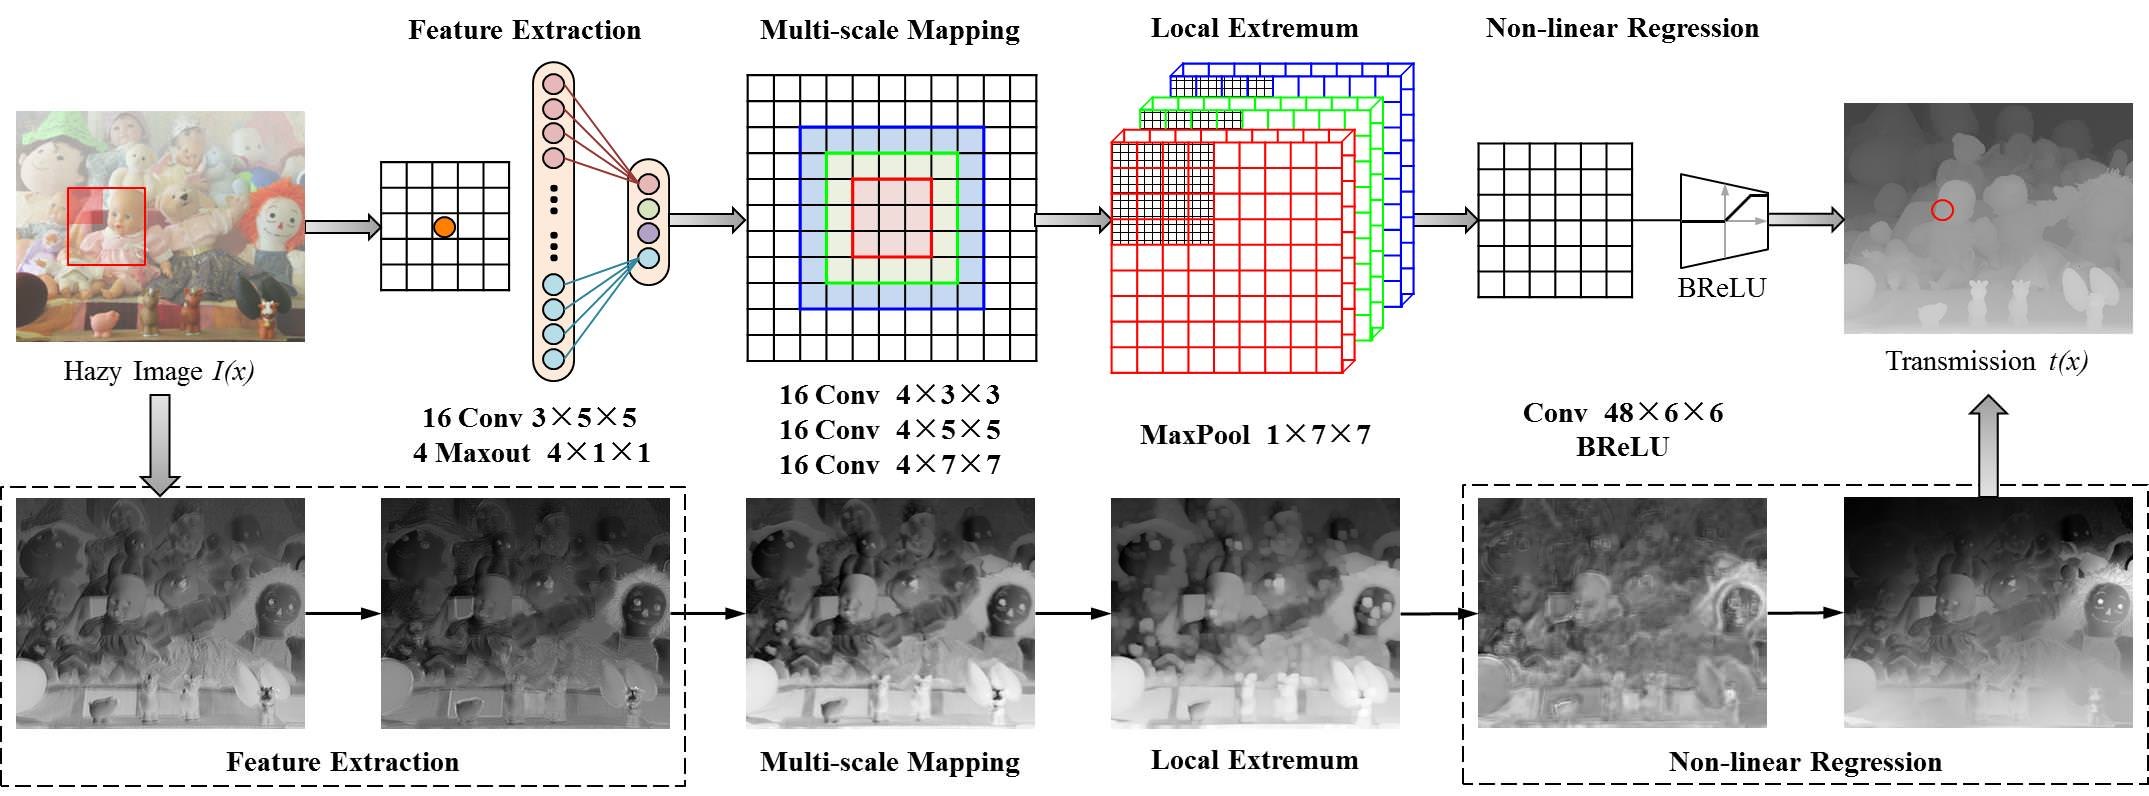
\includegraphics[width=\textwidth]{pic/pic4.png}
    \caption{DehazeNet的网络结构示意图}
\end{figure}


(1)输入层和特征提取层:
DehazeNet模型的输入层是尺寸为16*16 的有雾图像块。DehazeNet模型采用卷积层+激活层的结构来实现输入图像块的特征提取,其中,激活函数为最大输出单元(Maxout)。Maxout单元对输入特征图的通道进行分组,对每组特征图进行最大值操作。“卷积层+Maxout 激活函数”结构通过自动提取雾霾相关特征来代替传统去雾算法中先验特征的提取。

(2)多尺度映射层和局部极值层:
在DehazeNet模型中,为充分提取输入特征图中不同范围感受野的雾霾特征,采用不同卷积核大小的卷积层构建多尺度映射层。三组用于构建多尺度映射层的滤波器的卷积核大小分别为3*3 、5*5 和7*7 。并且,3组不同卷积核大小的滤波器个数均为16个。在传统去雾算法中,估计透射率值时一般假设有雾图像局部区域的透射率值是一致的。局部极值操作符合透射率的局部一致性假设,并可以有效抑制输出透射率图中的噪声。

(3)非线性回归层和输出层:
在非线性回归层,DehazeNet中采用新的双边纠正线性单元,该单元不仅能够保证对双边进行修正,还可以保证局部的线性。通过上述网络结构,可以得到输入图像块的透射率图。在DehazeNet中,大气光照值的估计基于暗通道先验理论,通过网络模型得到有雾图像的透射率图后,选择透射率图中较暗的像素值,再计算原有雾图像中这些像素点对应的强度,最大的强度值选为估计的大气光照值。最后,根据大气散射模型公式即可恢复清晰的无雾图像。

\subsection{基于多合一卷积网络AOD-Net的图像去雾算法}
基于先验知识构建的卷积神经网络模型,模型的输出为有雾图像的透射率图,并基于暗通道先验理论单独估计大气光照值。但是当有雾图像中物体背景和大气光接近时,可能会导致估计的大气光照值出现误差。并且,通过单独估计两个未知参数透射率值和大气光照值,再将两个参数的估计值代入大气散射模型中可能会进一步增大误差,影响去雾的效果。

为解决该问题,学者提出首个端到端的卷积神经网络模型AOD-Net 用于图像去雾,AOD-Net 模型的输出即为去雾后的清晰图像,并且无需单独估计透射率值和大气光照值。AOD-Net模型中关键的改进点是通过对大气散射模型公式进行变换,得到变换后的公式如下:
\begin{equation}J(x)=\frac{1}{t(x)} I(x)-A \frac{1}{t(x)}+A\end{equation}
将输入图像的透射率值$t(x)$和大气光照值$A$进行合并,可以得到:
\begin{equation}J(x)=K(x) I(x)-K(x)+b\end{equation}
其中, b为常数,从而可以得到:
\begin{equation}
    K(x)=\frac{{\frac{1}{t(x)}(I(x)-A)+(A-b)}}{I(x)-1}
\end{equation}

用这种方式,$\frac{1}{t(x)}$和$A$都被整合到$K(x)$中,$b$作为默认值为1的常数偏差。由于$K(x)$被独立于出$I(x)$,因此我们的目标是建立一个输入自适应的深度模型,并且最小化输出$J(x)$。
\begin{figure}[h]
    \centering
    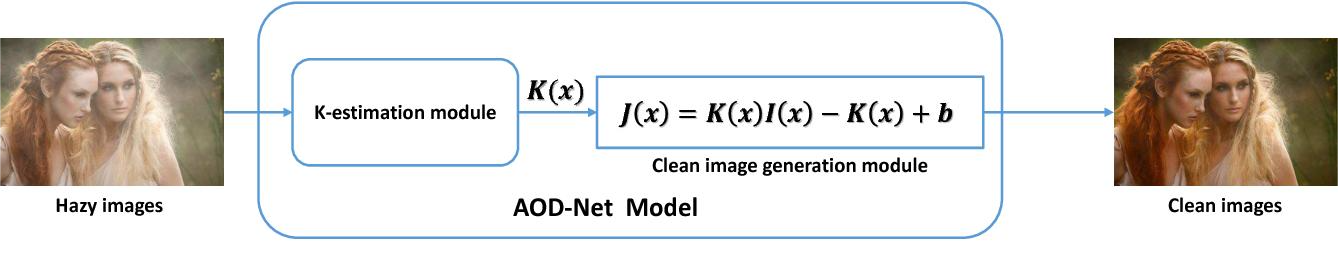
\includegraphics[width=\textwidth]{pic/pic5}
    \caption{AOD-Net的网络结构示意图}
\end{figure}

AOD-Net 模型中使用的损失函数是基于模型输出的无雾图像和实际有雾图像建立的,因此模型训练过程中损失函数值收敛较快,使用AOD-Net 模型进行单幅图像去雾所需的时间较少。


\section{总结}
目前针对有雾图像去雾的算法主要是从基于图像增强、图像复原和CNN 3个方向进行的。基于图像增强的方法不考虑有雾图像的形成过程,而是直接通过突出图像的细节,提高对比度等方式,从而使有雾图像看上去更加清晰。基于图像复原的方法则是追寻图像降质的物理过程,通过物理模型还原出清晰的图像。而基于CNN的方法则是利用神经网络强大的学习能力,寻找有雾图像与图像复原物理模型中某些系数的映射关系或者使用GAN,根据有雾图像还原出无雾的清晰图像。上述三类去雾算法对于雾天图像都有着明显的去雾效果,尽管其在实际生活中已经得到了广泛的应用,但下述几点仍有可能是今后图像去雾领域的研究重点和难点:
\begin{itemize}
    \item 更加真实的雾天图像数据集。采用神经网络进行去雾的算法在效果上好于图像增强和复原的方法,但是由于在自然界中很难拍摄到一组背景相同的有雾图像和无雾图像,因此目前训练神经网络所采用的数据集均是通过合成得到的,虽然能够在一定程度上拟合自然环境,但是仍然存在着一些差距。所以目前急需一种由在真实环境中获取到的具有相同背景的有雾图像和无雾图像构建的数据集,来提高神经网络去雾算法的鲁棒性和稳定性。
    \item 更加简便的去雾算法。目前各类算法能够有效去除单幅图像上的雾霾,但相对较好的算法都存在着时间复杂度高的问题,很难应用到视频去雾或者需求较多的复杂任务中去。
    \item 鲁棒性更强的去雾算法。上述算法都只对图像上存在的均匀的薄雾有较好的去雾效果,对于浓雾或者分布不均的团雾则效果较差,因此找到一种适用范围更广的去雾方法将会是一个极具挑战性的课题。
\end{itemize}

本文总结了目前常见的几种图像去雾算法以及在其基础上的改进算法,分析算法的优缺点及应用场景,希望图像去雾算法能在更多的领域得到应用。

\begin{thebibliography}{99}  


\bibitem{ref2}吴成茂.直方图均衡化的数学模型研究[J].电子学报,2013,41(03):598-602.
\bibitem{ref3}Pizer S M, Amburn E P, Austin J D, et al. Adaptive histogram equalization and its variations[J]. Computer vision, graphics, and image processing, 1987, 39(3): 355-368.
\bibitem{ref4}Land E H. The retinex[J]. American Scientist, 1964, 52(2): 247-264.
\bibitem{ref5}晁锐,张科,李言俊.一种基于小波变换的图像融合算法[J].电子学报,2004(05):750-753.
\bibitem{ref6}孙玉宝,肖亮,韦志辉,吴慧中.基于偏微分方程的户外图像去雾方法[J].系统仿真学报,2007(16):3739-3744+3769.
\bibitem{ref7}He K, Sun J, Tang X. Single image haze removal using dark channel prior[J]. IEEE transactions on pattern analysis and machine intelligence, 2010, 33(12): 2341-2353.
\bibitem{ref8}Cai B, Xu X, Jia K, et al. Dehazenet: An end-to-end system for single image haze removal[J]. IEEE Transactions on Image Processing, 2016, 25(11): 5187-5198.
\bibitem{ref9}Li B, Peng X, Wang Z, et al. An all-in-one network for dehazing and beyond[J]. arXiv preprint arXiv:1707.06543, 2017.
\bibitem{ref10}Zhang H, Patel V M. Densely connected pyramid dehazing network[C]//Proceedings of the IEEE conference on computer vision and pattern recognition. 2018: 3194-3203.
\bibitem{ref11}Liu X, Ma Y, Shi Z, et al. Griddehazenet: Attention-based multi-scale network for image dehazing[C]//Proceedings of the IEEE/CVF international conference on computer vision. 2019: 7314-7323.
\bibitem{ref12}Qin X, Wang Z, Bai Y, et al. FFA-Net: Feature fusion attention network for single image dehazing[C]//Proceedings of the AAAI Conference on Artificial Intelligence. 2020, 34(07): 11908-11915.

\end{thebibliography}

\end{document}